\documentclass[UTF8,10pt,a4paper]{ctexart}
\usepackage[margin=20mm,headheight=26pt]{geometry}
\usepackage{graphicx,xcolor,fancyhdr,booktabs,tabularx,enumitem,hyperref}
\definecolor{ink}{HTML}{12313B}\definecolor{teal}{HTML}{008F89}
\hypersetup{colorlinks=true,urlcolor=teal,linkcolor=teal,pdftitle={WorldGuard 提交材料}}
\setlength{\parindent}{0pt}\setlength{\parskip}{4pt}\linespread{1.12}
\setlist{nosep,leftmargin=1.5em}
\pagestyle{fancy}\fancyhf{}
\fancyhead[L]{\raisebox{-4pt}{
\includegraphics[height=8mm]{assets/logo.png}}\quad\textbf{\textcolor{ink}{WorldGuard}}}
\fancyhead[R]{\small 零界智行\quad U406}
\fancyfoot[L]{\footnotesize 本科生组 · 南京大学 / 东南大学}
\fancyfoot[R]{\footnotesize\thepage}
\renewcommand{\headrulewidth}{0.4pt}
\ctexset{section={format=\Large\bfseries\color{ink},beforeskip=12pt,afterskip=6pt},subsection={format=\large\bfseries\color{teal}}}
\newcommand{\cover}[2]{\vspace*{5mm}{\small\textcolor{teal}{WORLDGUARD / SUBMISSION 2026}}\par\vspace{4mm}{\huge\bfseries\color{ink}#1}\par\vspace{3mm}{\large #2}\par\vspace{4mm}\hrule\vspace{5mm}}
\newcommand{\note}[1]{\par\smallskip\noindent\colorbox{teal!7}{\parbox{0.95\linewidth}{\small #1}}\par\smallskip}
\begin{document}

\cover{WorldGuard 项目报告}{面向具身导航的故障测试、独立验收与恢复验证}
\textbf{参赛信息}\quad 本科生组 / U406 / 零界智行 / 队长：束宇涵\\
\textbf{方向}\quad C. Physical AI 与自主系统；C4. 无人系统与智能巡检\\
\textbf{材料版本}\quad 2026-10-15；基于已保存运行记录整理
\section{项目摘要}
WorldGuard 是面向室内导航策略的实验工作台。在单机器人二维几何仿真中，使用者上传受限 JSON 策略并描述测试目标；系统准备测试计划，经确认后执行正常、堵路或通道收窄等案例。Agnes Harness（AGH）组织模型与工具调用，确定性规划器生成路径，独立几何验收器在当前环境地图上检查整条路径的机器人足迹。发现失败后，可读取证据、更新地图并重新规划，或在未获得合格路径时停止。

作品的交付物包含地图快照、策略、路径、验收结果、恢复前后对照及工具事件。原始失败与恢复结果分别保存，便于评委复算。当前作品验证范围是二维几何导航，不包含真实机器人动力学或实机安全认证。
\section{问题来源与目标}
仓库环境变化会使旧地图上的可行路径失效；仅检查路径端点或中心线，也可能漏掉机器人身体在窄通道、障碍边角处的碰撞。开发者需要知道哪条路径、哪段线段、哪版地图出了问题，以及恢复动作是否真正满足原约束。
本项目的目标是把任务输入、故障注入、路径验收、反馈恢复与证据导出连接成可操作流程，使失败可见、结论可追溯、结果可复现。问题来源为工程场景抽象与合成实验，不冒充真实事故调查。
\section{核心方法与执行分工}
\begin{enumerate}
\item \textbf{任务准备：}解析目标与策略，生成固定场景和候选案例，用户确认后开始。
\item \textbf{AGH 编排：}真实模型调用受限 MCP 工具，查询候选、运行案例、审计路径、读取证据，决定恢复或结束。
\item \textbf{独立验收：}沿完整路径线段检查圆盘机器人扫掠区域与当前原始占用网格的关系，约束保持固定。
\item \textbf{反馈验证：}恢复使用更新地图，重新规划并再次验收；未得到合格路径则停止，停止不计为到达。
\item \textbf{交付证据：}保存输入、输出、地图版本和内容哈希，提供报告和复现样例。
\end{enumerate}

\section{代表性运行与结果}
以下为两次已完成的真实 Agnes 运行，非本轮重新执行，不是大样本统计。
\par
\begin{tabularx}{\linewidth}{Xrrrr}\toprule
场景 & 案例 & 原始通过 & 恢复通过 & 停止\\\midrule
复杂仓库（种子 90749）&3&1&2&0\\
窄通道（种子 11）&5&3&0&2\\\bottomrule
\end{tabularx}\par

两次运行模型标识均为 \texttt{agnes-3.0-flash}，记录分别为 19 与 23 次请求尝试。请求次数包含辅助请求，不能解释为全部成功或全部计费；完整 token 用量及费用未知。详细记录位于附件 04。
\begin{center}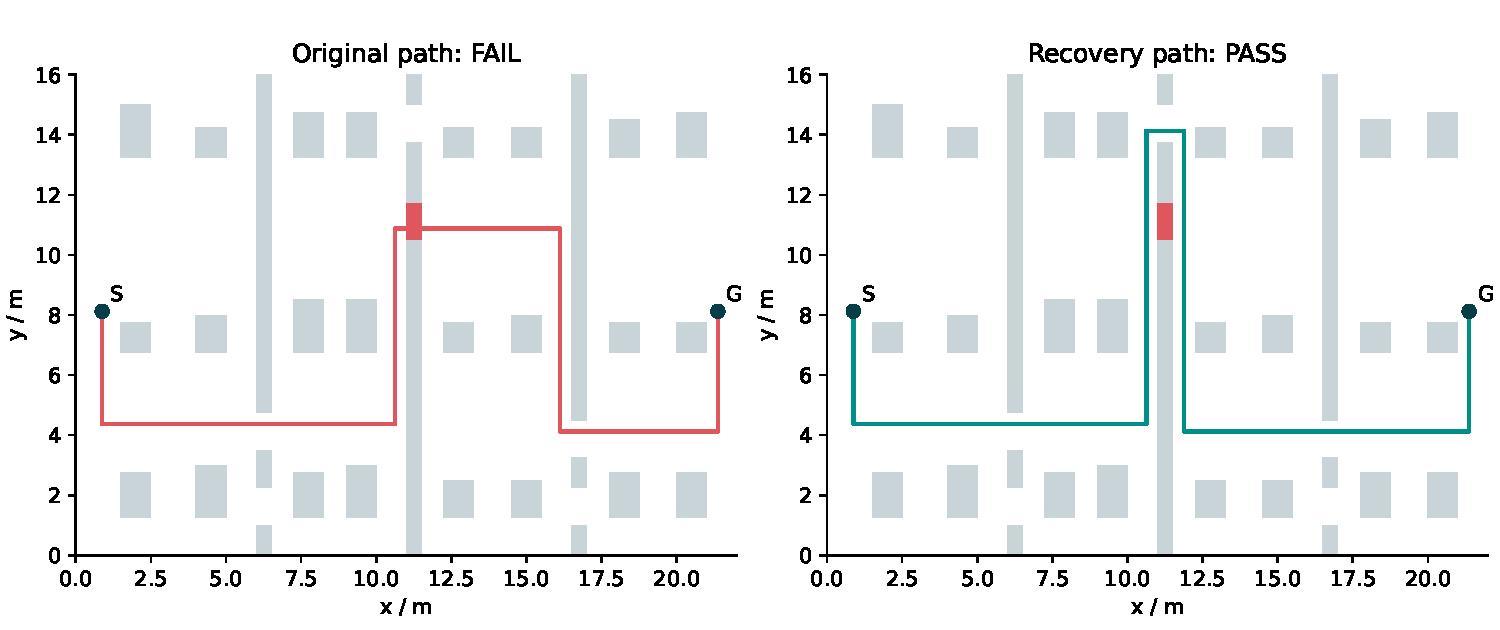
\includegraphics[width=\linewidth]{assets/verified-paths.pdf}\end{center}
\textbf{堵路案例 block\_route\_2：}原始路径最小剩余净空为 $-0.230$ m，独立验收不通过；恢复路径为 $0.145$ m，验收通过。路径长度从 41.5 m 增加至 48.0 m。图中红色格为新增障碍；图按附件真实网格和路径绘制。

\textbf{边界案例 pinch\_clearance\_2：}原始路径足迹不足，最小剩余净空为 $-0.105$ m；恢复阶段未找到合格路径，最终为停止。此结果不证明连续空间中不存在任何路径，也不应描述成恢复成功。
\section{技术特点与适用边界}
模型拥有工具动作的提议与编排能力，几何验收器负责路径是否满足明确约束的判定。验收凭据绑定地图、任务、约束、路径与验收器版本；任一内容变化均需重新验收。比较保留原始失败，避免用恢复通过覆盖初始问题。

策略参数比较、证据问答与反事实实验入口已在代码中实现，但这些增强功能不替代上述核心证据。当前尚无公平预算下的 Agent 增益对照，不能声称模型优于固定规则、达到普遍安全保证，或已经完成实机验证。
\section{团队与材料索引}
束宇涵：南京大学，地理科学，队长。何万里：南京大学，医学。郑博文：东南大学，电气。专业名称按成员提供信息记载；实际完成分工待本人核实，另见成员声明。

附件 02 为技术与运行指南，04 为执行与验证记录，05 为三类测试样例，06 为待成员签署声明与素材说明，07 为公开内容证明。视频由独立分支维护，已发布至 B站，链接见附件 07。

\end{document}
